%%% how to build
% pdflatex/xelatex/lualatex main.tex
% bibtex main
% pdflatex/xelatex/lualatex main.tex
% pdflatex/xelatex/lualatex main.tex

%% If you cannot use these templates, papers should be prepared in double column format,
%% with margins of 20mm, and a column width of 82mm.
%% Please use Times style font, size 10.5bp for body text, with no indents for new paragraphs.
%% Please use bolden Times style font, size 11bp for level 1 headings,
%% size 10.5bp for level 2 headings, and size 10.5bp for level 3 headings.
%% There should be a fixed space of 3mm before and 3mm after a level 1 heading,
%% 3mm before and 3mm after a level 2 heading, and 1mm before and 1mm after a level 3 heading,
%% unless headings appear immediately one after another, in which case a gap should not be left between them.
\documentclass{jcd}
\usepackage{float}
\usepackage{cuted}
\usepackage[ruled,linesnumbered]{algorithm2e}
\setlength{\algomargin}{4pt}
\SetAlCapHSkip{6pt}
% \def\nlstylewithcolon#1{\makebox[14pt][l]{\normalsize\kern4pt #1:}}
\def\NlSty#1{\makebox[14pt][l]{\kern3pt\normalsize#1:}}
% \SetNlSty{nlstylewithcolon}{}{}
\setlength{\algomargin}{22pt}
\SetKwFor{For}{for}{do}{end\ for}
\SetKwIF{If}{ElseIf}{Else}{if}{then}{else if}{else}{end\ if}

% \definecolor{url}{HTML}{467886}
\colorlet{url}{black}
\usepackage{hyperref}
\hypersetup{
  colorlinks  = true,
  % allcolors   = main,
  citecolor   = ref,
  linkcolor   = ref,
  urlcolor    = url,
  allcolors   = black,
}
\usepackage[numbered]{bookmark}
\usepackage{overpic}

%% you can use times fonts, if you use pdflatex/xelatex/lualatex.
% times fonts
\ifPDFTeX
\usepackage{newtxtext}
\usepackage{newtxmath}
\else
\usepackage{fontspec}
\setmainfont{Times New Roman}
\usepackage{newtxmath}
\fi

\renewcommand\sfdefault{\rmdefault}

\documentsetup{
  title={Templates for Journal of Control and Decision (Dec 2025)},
  history={Received 6 September 2025\\ Accepted ***},
  keywords={Keyword1; Keyword2; Keyword3; Keyword4; Keyword5; Keyword6.},
  authors={
    Givenname Familyname={a,b},
    Shiyi Pan={b},
    % Author c={a,c},
  },
  affiliations={
    a={State Key Laboratory of Synthetical Automation for Process Industries, Northeastern University, Shenyang, People's Republic of China},
    b={Alliance Manchester Business School, The University of Manchester, Manchester, UK},
    % c={National Engineering Technology Research Center for Metallurgical Industry Automation, Northeastern University, Shenyang, People's Republic of China},
  },
  contact-to=X. Author,
  contact-email={xAuthor@mail.neu.edu.cn},
  contact-address={State Key Laboratory of Synthetical Automation for Process Industries, Northeastern University, Shenyang 110819, People’s Republic of China.},
  notes={Supplemental data for this article (if any) can be accessed online at https://doi.org/10.1080/23307706.2025.2563818.},
}

\renewcommand{\textfraction}{0.1}
\renewcommand{\topfraction}{0.9}
\renewcommand{\dbltopfraction}{0.9}
\renewcommand{\bottomfraction}{0.5}
\renewcommand{\floatpagefraction}{0.7}

\theoremstyle{plain}
\theoremstyle{definition}
\newtheorem{theorem}{Theorem}[section]
\renewcommand{\thetheorem}{\arabic{section}.\arabic{theorem}}
\newtheorem{definition}{Definition}[section]
\renewcommand{\thedefinition}{\arabic{section}.\arabic{definition}}
\newtheorem{remark}{Remark}[section]
\renewcommand{\theremark}{\arabic{section}.\arabic{remark}}

\begin{document}

\maketitlepage
\arrayrulecolor{main} % set table line color

\begin{abstract}
This template is provided for authors submitting to the Journal of Control and Decision. It outlines the journal's formatting requirements, including title, abstract, keywords, main text, figure insertion, table preparation, references, and author biography. Authors are required to carefully review the instructions and insert the appropriate content in the designated sections. The template's layout parameters must not be altered.
\end{abstract}

\section{Introduction}

Journal of Control and Decision (JCD) provides templates in both Word and LaTeX formats. Please select the one that best suits your needs.

\subsection{Manuscript length}

Research articles should not exceed 14 pages, as a fee will be charged for any additional pages in the final manuscript, though this restriction does not apply to review articles.

\subsection{Submission anonymity}

T\/o facilitate our double-blind peer review process, all submissions (both initial and revised) should include two separate versions of the manuscript:

\begin{enumerate}
  \item	Manuscript-with author details: This file should include the complete list of all authors and their relevant information (names, affiliations, contact details). Please note that the designated first author cannot be altered post-submission, and co-first or co-corresponding authors are not permitted.
  \item	Manuscript-anonymous: This version is prepared for the reviewers and must not contain any information that could identify the authors or their institutions.
\end{enumerate}

When preparing the anonymous version, please ensure the following sections are blinded or have all identifying information removed:

\begin{itemize}
  \item Author details at the beginning of the article.
  \item Corresponding author information in the first page footer.
  \item Author biographies at the end of the document.
  \item Acknowledgments, funding information, and any other content that could reveal author identity.
  \item Note for revised submissions: The response letter to reviewers must also be submitted in an anonymized format.
\end{itemize}

\subsection{Permissions}

If your manuscript includes figures that have already been published elsewhere, you must obtain permission from the copyright owner(s) for both the print and online   format. Please be aware that some publishers do not grant electronic rights for free and that we will not be able to refund any costs that may have occurred to receive these permissions. In such cases, material from other sources should be used.

\section{Manuscript preparation and professional standards}

To ensure consistency and quality, all manuscripts must adhere to the following professional standards and formatting requirements.

\subsection{Overall manuscript standards}

The manuscript must be complete, including a title, author names and affiliations, abstract, keywords, main text, conclusion, Notes on Contributors, and references. The paper must demonstrate sound theoretical foundations, rigorous argumentation, substantial supporting evidence, and precise data. The writing should exhibit linguistic fluency, proper punctuation, and scholarly excellence, with a particular emphasis on academic rigor, innovation, and cutting-edge research perspectives.

\subsection{Main structure}

\textbf{Title:} The title should be concise and informative, accurately reflecting the scope and findings of the research.

\textbf{Abstract:} The abstract must comprehensively present four essential elements: Purpose, Methodology, Results, and Conclusions. For English abbreviations, provide the full term upon first use for less common acronyms. Widely recognized abbreviations (e.g., PID, LMI, GA, T-S, MIMO) may be used without expansion.

\textbf{Keywords:} Provide 4 to 8 keywords that accurately represent the core content and subject matter of the article.

\textbf{Introduction:} The introduction should concisely articulate the research background and current status. Please avoid extensive mathematical formulations and detailed theorem-related content in this section.

\textbf{Main text:} The main text should be formatted according to the journal's template. This is a double-column layout using 10.5 pt font. These settings are mandatory and must not be altered.

\textbf{Conclusion:} The conclusion should summarize the key findings of the study and their implications.

\textbf{Funding:} Include if applicable.

\textbf{Acknowledgment:} Include if applicable.

\textbf{Notes on contributors:} Author biographies should be formatted according to the example provided in the template.

\textbf{References:} References must be listed in the order of their appearance in the text. Please follow the formatting style detailed in the template.


\section{Author information}

\subsection{Initial submission}

When submitting your initial draft, please ensure that all authors are added to the submission system. Please note that the designated first author and first affiliation cannot be modified after the submission is finalized.

\subsection{Final manuscript requirements}

For the final manuscript, you should provide a colored photograph and a biography for each author.

\textbf{Author photograph:}
\begin{itemize}
  \item \textbf{Pixel dimensions:} 300 (width) $\times$ 425 (height)
  \item \textbf{Minimum resolution:} 300 DPI
  \item \textbf{File size:} Please adhere to the maximum file size limit specified in the submission system.
\end{itemize}

\textbf{Author biography:} The biography should follow the format and style of the example at the end of this template. It should be concise and written in the third person, typically covering educational background, current position, and primary research interests.


\section{Figures and Tables}

\subsection{Figure guidelines}

To ensure high-quality reproduction in both print and online formats, please adhere to the following guidelines when preparing figures for your manuscript.

\subsubsection{General quality and composition}

All figures should be properly arranged with appropriate dimensions, clear lines, and concise text and symbols.

Figures should be aesthetically pleasing and professionally presented.

\subsubsection{Formatting and labels}

\textbf{Figure captions:} The main figure caption (e.g., “Figure 1. Velocity tracking…”) should be 9.5 pt, left-aligned. Please refer to \autoref{fig-1} for an example.

\begin{figure}[H]
  \centering
  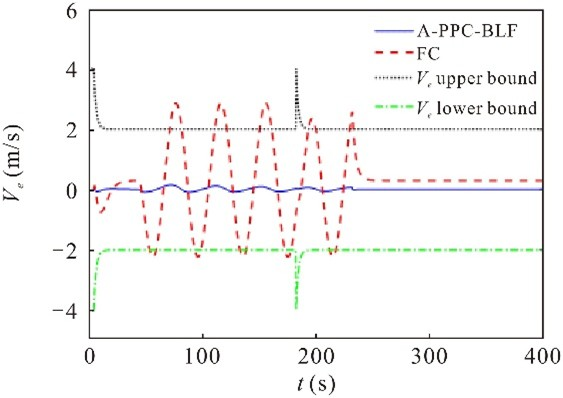
\includegraphics{figures/_fig1}
  \caption{Velocity tracking and velocity tracking error.}\label{fig-1}
\end{figure}

\textbf{Subfigure labels:} Labels for subfigures (e.g., (a) Normalized…) should be 8.5 pt, centered below each respective subfigure, and fully editable. Please refer to Figure 2 for an example.

\textbf{Text within figures:} To ensure consistency, we strongly recommend using Times New Roman within your figures. Variables should be italicized, while constants and units should be in regular (roman) font.

\textbf{Legends:} Legends should not obscure data lines or interfere with the clear expression of information. The preferred placement is inside the figure’s bounding box. If this is not possible without affecting clarity, place the legend to the right of or below the figure.

\begin{figure}[H]
  \centering
  \subcaptionbox{Normalized mutual information (NMI)}
    [\linewidth]{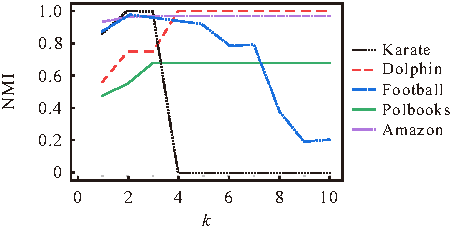
\includegraphics[width=\linewidth]{figures/_fig2-a}}

  \vspace{12pt}

  \subcaptionbox{Modularity ($Q$)}
    [\linewidth]{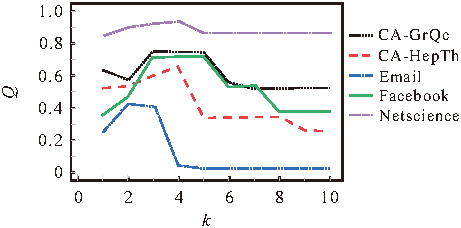
\includegraphics[width=\linewidth]{figures/_fig2-b}}
  \caption{Performance of the CDWD algorithm.}\label{fig-2}
\end{figure}

\subsubsection{Color considerations}

Please note that the journal is printed in black and white. Therefore, figures should be designed to be clearly legible without relying on color to differentiate data.
The use of color is permitted for the online version of the article, but it should be used to enhance, not replace, clear black-and-white distinction.

\subsection{Table guidelines}

Tables should be simple and well-defined, preferably using the three-line format (i.e., tables without vertical lines and only three horizontal lines, except in special circumstances). Table titles should be positioned directly above the table. All parameters in tables must indicate their units, as shown in \autoref{tab-1}. Overly lengthy tables may span the full width of the page.

\begin{table}[H]
  \footnotesize
  \caption{Initial state parameters of the tanker aircraft.}\label{tab-1}
  \begin{tabularx}{\linewidth}{@{} l *{4}{>{\centering\arraybackslash}X}}
    \toprule
    Quadrant & I & II & III & IV\\ \midrule
    Position(km) & (40,0,7) & (100,10,6.8) & (70,50,5) & ($-$20,40,8)\\
    Velocity(m·s\textsuperscript{$-$1}) & 200 & 220 & 180 & 220\\
    Declination(\textdegree) & 90 & 0 & 180 & 90\\
    Inclination(\textdegree) & 15 & 0 & 0 & $-$15\\ \bottomrule
  \end{tabularx}
\end{table}

\textbf{Format:} Tables should be simple and clearly defined. We strongly recommend using the three-line format. This format should be used unless special circumstances require an alternative.

\textbf{Title:} The table title must be positioned directly above the table. It should be 9.5 pt and left-aligned.

\textbf{Content:} All parameters within the table must have their units clearly indicated. The text within the table should be 8 pt.

\textbf{Layout:} To ensure readability, overly lengthy tables may be formatted to span the full width of the page.

Please refer to the following examples:

\arrayrulecolor{black}
\begin{table}[H]
  \linespread{1}\renewcommand\arraystretch{1}\footnotesize
  \setlength{\tabcolsep}{2pt}
  \def\aboverulesep{0pt}\def\belowrulesep{0pt}
  \setlength{\doublerulesep}{.7bp}\setlength{\arrayrulewidth}{.5bp}
  \renewcommand{\tabularxcolumn}[1]{m{#1}}
  \caption{Primary symbols and their corresponding definitions.}\label{tab-2}
  \begin{tabularx}{\linewidth}
      {@{} >{$}l<{$} >{\raggedright\arraybackslash}X || >{$}c<{$} >{\raggedright\arraybackslash}X}
    \hline
    \Gape[4pt]{\textbf{Symbols}} & \multicolumn{1}{c||}{\textbf{Definition}} & \textbf{Symbols} & \multicolumn{1}{c}{\textbf{Definition}}\\
      \cmidrule(r{1.2pt}){1-2}\cmidrule(l{-.50pt}){3-4}
    M & \gape[t]{Particle population size} & m & $m$th particle\\
    H_{\mathrm{max}} & Maximum iterations & h & $h$th iteration\\
    R' & Dimension of the search space & r' & $r'$th dimension\\
    x & Position of particle $p_m$ & v & Velocity of particle $p_m$\\
    W & Inertia weight & \Delta w & Inertia weight increment\\
    c_1 & Individual experience acceleration factor & c_2 & Social experience acceleration factor\\
    \delta_c & Commanded steering angle & \delta_a & Actual steering angle\\
    x_c & Control input & y_a & Actual output\\ \hline
  \end{tabularx}
\end{table}
\arrayrulecolor{main}

\section{Equations and other examples}

All equations, algorithms, theorems, remarks, proofs, and hypotheses within the main text should be formatted as part of the body content, set in 10.5pt font size.

\begin{strip}
% \begin{table}[b]
  \centering\footnotesize
  \setlength{\tabcolsep}{10pt}
  \renewcommand{\captionwidth}{.805\textwidth}
  \captionof{table}{Model performance comparison.}
  \begin{tabular}{@{} l *{6}{c}}
    \arrayrulecolor{main}
    \toprule
    \arrayrulecolor{gray}
    & \multicolumn{2}{c}{$I$ = 1.8 A} & \multicolumn{2}{c}{$I$ = 1.35 A} & \multicolumn{2}{c}{$I$ = 0.9 A}\\
      \cmidrule(r{3pt}){2-3}\cmidrule(l{3pt}r{3pt}){4-5}\cmidrule(l{3pt}){6-7}
    Model & RMSE(Ah) & MAPE(\%) & RMSE(Ah) & MAPE(\%) & RMSE(Ah) & MAPE(\%)\\ \midrule
    Physical & 0.245 & 32.863 & 0.093 & 8.715 & 0.235 & 27.114\\
    LSTM & 0.013 & 1.634 & 0.044 & 4.067 & 0.007 & 0.759\\
    CNN & 0.003 & 0.411 & 0.026 & 2.400 & 0.009 & 1.016\\
    Hybrid (MLP) & 0.018 & 2.391 & 0.083 & 7.770 & 0.156 & 17.956\\
    \arrayrulecolor{main}
    Hybrid (KAN) & \bfseries 0.002 & \bfseries 0.278 & \bfseries 0.004 & \bfseries 0.329 & \bfseries 0.006 & \bfseries 0.652\\ \bottomrule
  \end{tabular}
% \end{table}
\end{strip}

\subsection{Equation guidelines}

Equations should be centered on the column, with their corresponding numbering aligned to the right margin.
\begin{equation}
% CL_{C_{k}} =1-\sum_{t=1}^{n_{k}}\theta_t
% \raisebox{-.2\height}{$\dfrac{\displaystyle 2\times\sum_{i=1}^{n-1}\sum_{j>i}^n\left|t_{ij}^{(k)}-t_{ij}^{(C)}\right|}{\displaystyle n\times(n-1)}$}
% CL_{C_{k}} =1-\sum_{t=1}^{n_{k}}\theta_{t 
% \dfrac{\displaystyle 2\times\sum_{i=1}^{n-1}\sum_{j>i}^n\left|t_{ij}^{(k)}-t_{ij}^{(C)}\right|}{\displaystyle n\times(n-1)}}
CL_{C_{k}} =1-\sum_{t=1}^{n_{k}}\theta_t
\dfrac{\displaystyle 2\times\sum_{i=1}^{n-1}\sum_{j>i}^n\left|t_{ij}^{(k)}-t_{ij}^{(C)}\right|}{\displaystyle n\times(n-1)},
\end{equation}
\begin{equation}
  \begin{aligned}
J_{T_n}(u_n)-J(\nu) &=\int_0^{T_n}\left(\frac{r}{p}{\left|u_n(t)\right|}^p+{\left\|y_n(t)\right\|}^q\right)\mathrm{d}t \\
 &\phantom{=} -\int_0^{+\infty}\left(\frac{r}{p}|u_n(t)|^p+\|y_n(t)\|^q\right)\mathrm{d}t \\
 &= J_{T_n}(u_n)-J_{T_n}(\nu) \\
 &\phantom{=} -\int_{T_n}^{+\infty}\left(\frac{r}{p}|u_n(t)|^p+\|y_n(t)\|^q\right)\mathrm{d}t\leq0,
  \end{aligned}
\end{equation}
\begin{equation}\makegapedcells\setcellgapes{2pt}\setlength{\arraycolsep}{3.2pt}
  \begin{aligned}
  E_{\alpha}(J_{k},t) & =E_\alpha(\lambda_k,t) \\
  & =
  \begin{bmatrix}
  1 & \dfrac{t^\alpha}{\alpha} & \dfrac{t^{2\alpha}}{\alpha^22!} & \dfrac{t^{3\alpha}}{\alpha^33!} & \cdots & \dfrac{t^{(n_k-1)\alpha}}{\alpha^{n_k-1}(n_k-1)!} \\
  0 & 1 & \dfrac{t^\alpha}{\alpha} & \dfrac{t^{2\alpha}}{\alpha^22!} & \cdots & \dfrac{t^{(n_k-2)\alpha}}{\alpha^{n_k-2}(n_k-2)!} \\
  0 & 0 & 1 & \dfrac{t^\alpha}{\alpha} & \ddots & \dfrac{t^{(n_k-3)\alpha}}{\alpha^{n_k-3}(n_k-3)!} \\
  \vdots & \vdots & \ddots & \ddots & \ddots & \vdots \\
  0 & 0 & \cdots & 0 & \ddots & \dfrac{t^\alpha}{\alpha} \\
  0 & 0 & \cdots & 0 & 0 & 1
  \end{bmatrix}
  \end{aligned}.
\end{equation}

\subsection{Other examples}

For algorithms, a three-line table is the recommended format. If a three-line table is not used, the steps should be labeled sequentially (e.g., “Step 1:”, “Step 2:”).

% \begin{list}{}{\setlength{\algomargin}{6pt}%
%   \setlength{\leftmargin}{\algomargin}\rightmargin\leftmargin
%   \setlength{\parindent}{0pt}\listparindent\parindent
%   \setlength{\topsep}{0pt}\setlength{\parsep}{0pt}\setlength{\partopsep}{0pt}
% }\item
% \begin{tabbing}
% \hspace{-\algomargin}\rule{\dimeval{\linewidth+2\algomargin}}{.5pt}\hspace{-\algomargin}\\
% \parbox[b]{\linewidth}{\textbf{Algorithm 1:} Fractional-order online gradient descent algorithm with constraints.}\\[-10pt]
% \hspace*{-\algomargin}\rule{\dimeval{\linewidth+\algomargin+\algomargin}}{.5pt}\hspace{-\algomargin}\\
% 99:\;\=for\;\=\quad\=\ \=\kill
% 1: \> Initialize $\alpha,\delta,\eta_0,x_0\in \chi\in \mathbb{R}^d$\\
% 2: \> \textbf{for} $t=0$ {\normalfont to} $T$ \textbf{to}\\
% 3: \>\> \textbf{if} $t=0$ \textbf{then}\\
% 4: \>\>\> $y_1=x_0-\eta_0\nabla f_0(x_0)$\\
% 5: \>\>\> $\displaystyle x_1=\prod_{\chi} y_1$\\
% 6: \>\> \textbf{else}\\
% 7: \>\>\> $\displaystyle y_{t+1}=x_t-\eta_t\frac{\nabla f_t(x_t)}{\varGamma(2-\alpha)}(\Vert x_t-x_{t-1}\Vert+\delta)^{1-\alpha}$\\
% 8: \>\>\> $\displaystyle x_{t+1}=\prod_{\chi} y_{t+1}$\\
% 9: \>\> \textbf{end if}\\
% 10: \> \textbf{end for}\\
% 11: \> \textbf{return} $x_{{\scriptscriptstyle T}+1}$\\[-10pt]
% \hspace*{-\algomargin}\rule{\dimeval{\linewidth+\algomargin+\algomargin}}{.5pt}\hspace{-\algomargin}
% \end{tabbing}
% \end{list}

% \usepackage{algorithm2e}
\enlargethispage{5pt}
\begin{algorithm}
\SetAlgoNoLine
Initialize $\alpha,\delta,\eta_0,x_0\in \chi\in \mathbb{R}^d$

\For{$t=0$ {\normalfont to} $T$}{
  \eIf{$t=0$}
    {$y_1=x_0-\eta_0\nabla f_0(x_0)$\\
    $\displaystyle x_1=\prod_{\chi} y_1$}
    {$\displaystyle y_{t+1}=x_t-\eta_t\frac{\nabla f_t(x_t)}{\varGamma(2-\alpha)}(\Vert x_t-x_{t-1}\Vert+\delta)^{1-\alpha}$\kern-20pt\\
    $\displaystyle x_{t+1}=\prod_{\chi} y_{t+1}$}
}

\KwRet{$x_{{\scriptscriptstyle T}+1}$}
\caption{Fractional-order online gradient descent algorithm with constraints.}
\end{algorithm}

Other elements such as Theorems, Remarks, Proofs, and others should follow the examples provided below.

\begin{theorem}\label{theorem:3.1}
For the 2-D vehicular platooning system (1) with the actuator faults (4), by exploiting the compound prescribed-time fault observers as, (9) -- (13) the compound faults are estimated in the prescribed time with zero estimation errors by choosing the appropriate constants $\alpha_{v1,i}$ , and $\alpha_{\varphi1,i}$ .
\end{theorem}

\begin{remark}
In the improved prescribed-time compound fault observers in (9) and (10), by selecting the appropriate constants $\alpha_{v1,i}$ , and $\alpha_{\varphi1,i}$ , the compound fault observers can ensure faster convergence rate with a prescribed time $T_{a}>0$ .
\end{remark}

\begin{proof}
The user's secret $x_i$ is generated locally and never exposed to the KGC. The KGC only provides $D_{v_i}=r_i+x\beta_i$ , which is insufficient to compute $x_i$. Concluding KGCs cannot solve $x_i$ from $PK_i=x_iK+D_{v_i}P$ due to ECDLP.\qedhere
\end{proof}


\section{Notes on contributors}

\vspace{-2mm}

\begin{contributor}{First Author1}{author1.png}% arg 1: author, arg 2: portrait pic
received a B.S. degree in electrical and automation from Qingdao
University, Qingdao, China, in 2007 and the M.S. and Ph.D. degrees in control theory
and control engineering from Northeastern University, Shenyang, China, in
2009 and 2014, respectively. He is currently a Professor at the School of
Information and Control Engineering, and the Ministry of Education
Engineering Research Center of Intelligent Control for
Underground Space, China University of Mining and Technology,
where he is also a Professor at the Institute of Artificial
Intelligence, China University of Mining and Technology. His current research
interests include modelling and control of complex industrial processes.
\end{contributor}


% remove the number of sections
\backmatter

\section{References}
% \usepackage{natbib,apacite}

\normalsize

Please ensure all cited sources are from formally published works, such as journals, books, or conference proceedings. References should be numbered sequentially in the order of appearance and formatted according to APA-7. For detailed specifications, please refer to the \href{https://files.taylorandfrancis.com/tf_APA.pdf}{reference style guide}.

Please refer to the following examples:
%\citep{Li2025EcoDriving,Wang2025PowerSeries,Franklin2019DigitalControl,Sklar2001DigitalComm,Kilbas2003FractionalDE,Wang2024NRBOSVM}:

\urlstyle{rm}
% \bibliography{reference.bib}

\vspace{2pt}
{\bfseries\fontsize{9.5bp}{12bp} Journal articles}\par
\vspace{2pt}
\begin{thebibliography}{}
\bibitem [\protect \citeauthoryear {%
  Li%
  \ \protect \BOthers {.}}{%
  Li%
  \ \protect \BOthers {.}}{%
  {\protect \APACyear {2025}}%
  }]{%
  Li2025EcoDriving}
  \APACinsertmetastar {%
  Li2025EcoDriving}%
  \begin{APACrefauthors}%
  Li, S.%
  , Wang, J.%
  , Pan, J.%
  , Chen, C.%
  , Xu, Q.%
  \BCBL {}\ \BBA {} Li, K.%
  \end{APACrefauthors}%
  \unskip\
  \newblock
  \APACrefYearMonthDay{2025}{}{}.
  \newblock
  {\BBOQ}\APACrefatitle {Eco-driving control of intelligent and connected vehicles through multiple signalised intersections under cloud control system} {Eco-driving control of intelligent and connected vehicles through multiple signalised intersections under cloud control system}.{\BBCQ}
  \newblock
  \APACjournalVolNumPages{Journal of Control and Decision}{12}{6}{976--993}.
  \newblock
  \begin{APACrefDOI} \doi{10.1080/23307706.2025.2500057} \end{APACrefDOI}
  \PrintBackRefs{\CurrentBib}
\bibitem [\protect \citeauthoryear {%
  J.~Wang%
  , Bobtsov%
  , Aranovskiy%
  , Efimov%
  \BCBL {}\ \BBA {} Pyrkin%
  }{%
  J.~Wang%
  \ \protect \BOthers {.}}{%
  {\protect \APACyear {2025}}%
  }]{%
  Wang2025PowerSeries}
  \APACinsertmetastar {%
  Wang2025PowerSeries}%
  \begin{APACrefauthors}%
  Wang, J.%
  , Bobtsov, A.%
  , Aranovskiy, S.%
  , Efimov, D.%
  \BCBL {}\ \BBA {} Pyrkin, A.%
  \end{APACrefauthors}%
  \unskip\
  \newblock
  \APACrefYearMonthDay{2025}{}{}.
  \newblock
  {\BBOQ}\APACrefatitle {Power series for noise attenuation in linear regression parameter estimation} {Power series for noise attenuation in linear regression parameter estimation}.{\BBCQ}
  \newblock
  \APACjournalVolNumPages{Journal of Control and Decision}{}{}{1--8}.
  \newblock
  \begin{APACrefDOI} \doi{10.1080/23307706.2025.2587081} \end{APACrefDOI}
  \PrintBackRefs{\CurrentBib}
\end{thebibliography}

\vspace{2pt}
{\bfseries\fontsize{9.5bp}{12bp} Books}\par
\vspace{2pt}
\begin{thebibliography}{}
\bibitem [\protect \citeauthoryear {%
  Franklin%
  , Powell%
  \BCBL {}\ \BBA {} Workman%
  }{%
  Franklin%
  \ \protect \BOthers {.}}{%
  {\protect \APACyear {2019}}%
  }]{%
  Franklin2019DigitalControl}
  \APACinsertmetastar {%
  Franklin2019DigitalControl}%
  \begin{APACrefauthors}%
  Franklin, G\BPBI F.%
  , Powell, J\BPBI D.%
  \BCBL {}\ \BBA {} Workman, M\BPBI L.%
  \end{APACrefauthors}%
  \unskip\
  \newblock
  \APACrefYear{2019}.
  \newblock
  \APACrefbtitle {Digital Control of Dynamic Systems} {Digital control of dynamic systems}\ (\PrintOrdinal{3}\ \BEd).
  \newblock
  \APACaddressPublisher{}{Ellis-Kagle Press}.
  \PrintBackRefs{\CurrentBib}
\bibitem [\protect \citeauthoryear {%
  Kilbas%
  , Srivastava%
  \BCBL {}\ \BBA {} Trujillo%
  }{%
  Kilbas%
  \ \protect \BOthers {.}}{%
  {\protect \APACyear {2003}}%
  }]{%
  Kilbas2003FractionalDE}
  \APACinsertmetastar {%
  Kilbas2003FractionalDE}%
  \begin{APACrefauthors}%
  Kilbas, A\BPBI A.%
  , Srivastava, H\BPBI M.%
  \BCBL {}\ \BBA {} Trujillo, J\BPBI J.%
  \end{APACrefauthors}%
  \unskip\
  \newblock
  \APACrefYearMonthDay{2003}{}{}.
  \newblock
  {\BBOQ}\APACrefatitle {Fractional differential equations: A emergent field in applied and mathematical sciences} {Fractional differential equations: A emergent field in applied and mathematical sciences}.{\BBCQ}
  \newblock
  \BIn{} G.~Litvinchuk\ (\BED), \APACrefbtitle {Factorization, Singular Operators and Related Problems} {Factorization, singular operators and related problems}\ (\BPGS\ 151--173).
  \newblock
  \APACaddressPublisher{}{Springer}.
  \PrintBackRefs{\CurrentBib}
\end{thebibliography}

\vspace{2pt}
{\bfseries\fontsize{9.5bp}{12bp} Conference proceedings}\par
\vspace{2pt}

\begin{thebibliography}{}
\bibitem [\protect \citeauthoryear {%
  M.~Wang%
  , Huo%
  \BCBL {}\ \BBA {} Jia%
  }{%
  M.~Wang%
  \ \protect \BOthers {.}}{%
  {\protect \APACyear {2024}}%
  }]{%
  Wang2024NRBOSVM}
  \APACinsertmetastar {%
  Wang2024NRBOSVM}%
  \begin{APACrefauthors}%
  Wang, M.%
  , Huo, K.%
  \BCBL {}\ \BBA {} Jia, Q.%
  \end{APACrefauthors}%
  \unskip\
  \newblock
  \APACrefYearMonthDay{2024}{}{}.
  \newblock
  {\BBOQ}\APACrefatitle {Rolling bearings fault diagnosis method based on {NRBO}-{SVM}} {Rolling bearings fault diagnosis method based on {NRBO}-{SVM}}.{\BBCQ}
  \newblock
  \BIn{} \APACrefbtitle {2024 IEEE International Conference on Mechatronics and Automation (ICMA)} {2024 ieee international conference on mechatronics and automation (icma)}\ (\BPGS\ 620--625).
  \newblock
  \APACaddressPublisher{}{IEEE}.
  \newblock
  \begin{APACrefDOI} \doi{10.1109/ICMA61710.2024.10632999} \end{APACrefDOI}
  \PrintBackRefs{\CurrentBib}
\end{thebibliography}

\vfil
\balance


\switchonecolumn
\section{Appendix (if any)}

\end{document}